\chapter{Background}
\label{cha:background}
This thesis investigates a middleware for realising secure and protected aggregation of data exposed through the Solid protocol. Section \ref{sec:solid} introduces the basic concepts of Solid, while section \ref{sec:macaroons} introduces some necessary background knowledge on macaroons, a novel type of access token.

\section{Solid}
\label{sec:solid}

\subsection{Introduction}
\begin{quote}{Tim Berners-Lee}
    The Semantic Web is not a separate Web but an extension of the current one, in which information is given well-defined meaning, better enabling computers and people to work in cooperation.
\end{quote}

\noindent In 2001, Sir Tim Berners-Lee - the inventor of the world-wide web - published an article in \textit{Scientific American} entitled `The semantic Web' \citep{semantic-web}. It envisioned a future where the Web was not just a collection of pages with meaningless links to each other, but a smart Web, where objects and relations have well-defined meanings.

Today, most resources accessible on the Web are meant for people to read, understand and process, but they are not adapted to automated processing by software agents. Computers can read information and format it correctly, but they lack a unified way to interpret the information: there is no way to process the \textit{semantics}. The Semantic Web is a proposal to combat this problem. The Semantic Web tries to solve this problem by extending the current Web with new, compatible standards and protocols to attach computer-readable meaning to information available on the Web.

Currently, markup languages such as XML enable users to arbitrarily structure documents the way they want it (e.g. using a tag called \texttt{<book>} and a tag called \texttt{<isbn>}). They then write software that parses this by telling the software that \texttt{<book>} means "book" and \texttt{<isbn>} means "isbn". However, other users may use different terms (e.g. \texttt{<isbn13>} instead of \texttt{<isbn>}), making information not universally parsable. 

\noindent The Semantic Web introduces the \gls{RDF}, which encodes structure and information in sets of triples: a subject, a predicate and an object. These triples then create a knowledge graph called an RDF graph, where predicates relate subjects to objects. The objects in one triple can then be the subjects in another one. The figure below illustrates an example, where Tokyo is the subject of a linked data triple, and two predicates relate it to its area and the country it resides in. The object, Japan, may then be the subject of other RDF graphs, relating it for example to its population.

\begin{figure}[H]
    \centering
    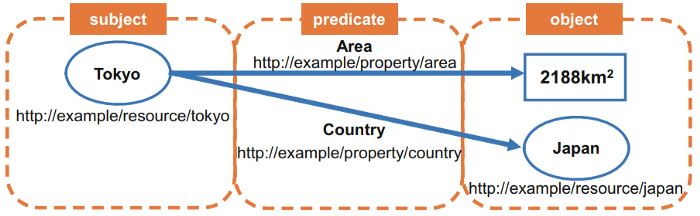
\includegraphics[width = 0.9\textwidth]{images/background/linked-data.png}
    \caption{\gls{RDF} representation of the city Tokyo, with predicates relating it to its area and its country. Source: \citet{generating-pva}}
    \label{fig:linked-data}
\end{figure}

\noindent Subjects, predicates and objects are all identified by a URI, making them universal, and allowing anyone to define new predicates\footnote{Unless they are literals, such as the area in the example}. In this manner, webs of information are formed between related objects using definitions that can be found and understood by everyone.

This does not completely solve the problem, however. It is possible that multiple definitions exist for essentially the same object. To resolve this, the Semantic Web introduces a third component: ontologies. Ontologies are documents that formally define the relations among terms \citep{semantic-web}. A widely-used ontology is called \textit{foaf}\footnote{\url{ http://xmlns.com/foaf/spec/}} (friend-of-a-friend): it is used to describe relationships between people.

\gls{RDF}, however, is only something conceptual (a collection of subject, predicate and object). If we want to actually use it, we need to store \gls{RDF} in documents. This is possible in multiple ways, i.e., multiple representation formats exist. The most popular ones are Turtle \citep{turtle} and JSON-LD \citep{jsonld}. Turtle has the advantage that it allows defining prefixes at the top of the file, which are aliases for the long URIs needed to relate the subjects/predicates/objects. If you want to talk about the foaf ontology, you can define at the top of your file:

\mint{cucumber}|@prefix foaf <http://xlmns.com/foaf/0.1/>|

\noindent You can then use \mintinline{cucumber}|foaf| in the rest of your turtle file, instead of\\ \mintinline{cucumber}|<http://xlmns.com/foaf/0.1/>|. This makes it very human-readable compared to other formats. Additional existing formats are \gls{RDF}/XML and N-Triples, but they are less common.

\subsection{The Solid Protocol}
\begin{quote}{\href{https://solidproject.org}{solidproject.org}}
    Solid is a proposed set of conventions and tools for building \textit{decentralized applications} based on Linked Data principles.
\end{quote}
% TODO pod as abbreviation: add to index?

\noindent Solid \citep{solid} is a proposed W3C specification that wishes to decentralize the web by giving people control over their data. Solid aims to realize this by giving people an online datastore called a \textit{pod} (personal online datastore). Users can then login to applications using an authentication mechanism provided by Solid, and the application can in turn access data stored in the user's pod.

By storing all the data inside the user's pod instead of on the application server, the user retains complete control over his data. He can flexibly choose what data to share with what applications. Furthermore, storing the data in a pod reduces vendor lock-in: when the user wishes to switch from one service to another, he can simply give the new application access to the data he already possesses. 

In Solid, there are two types of resources: linked and non-linked data resources. Non-linked data resources are the usual kinds of data that we access on the web right now (binary, text, images, ...), while linked data follows the 
 \gls{RDF} specifications by using a content representation such as Turtle. These linked-data standards follow the principles of the Semantic Web.

\subsection{Authentication}
Needless to say, some of the data stored in a user's pod should be protected; such that not every agent on the web can read it. To achieve this goal, Solid needs an authentication mechanism. Formally, authenticating a user is defined as the act of verifying a user's claimed identity.\todo{cite ref (comes from Solid)} As such, two components are needed: a way to form identities, and a way to verify that a user possesses an identity.

\subsubsection{Identities}
Identities in solid (both for users and other agents) follow the WebID standard \citep{webid}, where URIs act as universal identifiers. An example WebID is:

\begin{center}
   \texttt{https://jessegeens.solidcommunity.net/profile/card\#me}\\
\end{center}

\noindent These WebID URIs can identify several things: users, software agents, or other things (even if they do not exist on the web). The WebID URI references a WebID Profile Document. This document contains information about the agent who is the referent of the WebID URI. However, an important distinction must be made. When the \textit{\texttt{\#me}} is included in the URI (or more in general, the hashtag), this URI refers to an agent. When the hashtag is omitted, the URI refers to the document describing this agent.

\newpage
{\captionsetup{aboveskip=-0.2\normalbaselineskip}{
\begin{code}
\begin{minted}[linenos,tabsize=2,breaklines]{cucumber}
@prefix foaf: <http://xmlns.com/foaf/0.1/>.
@prefix solid: <http://www.w3.org/ns/solid/terms#>.

<>
    a foaf:PersonalProfileDocument;
    foaf:maker <http://localhost:3002/jesse/profile/card#me>;
    foaf:primaryTopic <http://localhost:3002/jesse/profile/card#me>.

<http://localhost:3002/jesse/profile/card#me>
    
    solid:oidcIssuer <http://localhost:3002/>;
    a foaf:Person.
\end{minted}
\caption{Example WebID profile document}
\label{listing:webid-profile}
\end{code}}}

%\begin{figure}
%    \begin{verbatim}

%    \end{verbatim}
%    \caption{Example WebID profile document}
%    \label{fig:webid-profile}
%\end{figure}

\subsubsection{Verifying identities}
While the WebID standard provides identities, it does not yet verify them. The actual authentication (or, verifying that the agent actually controls the WebID he claims to control) in Solid uses the WebID-OIDC protocol. This protocol draws inspiration from OAuth2 and from OpenID Connect. The workflow below, drawn from the WebID-OIDC repository, explains the basic mechanism of the protocol from the point-of-view of the user:

\begin{quote}{\href{https://github.com/solid/webid-oidc-spec}{webid-oidc-spec repository}}

    1. \textbf{Initial Request}: Alice (unauthenticated) makes a request to bob.example, receives a \texttt{HTTP 401 Unauthorized} response, and is presented with a 'Sign In With...' screen.\\
    
    2. \textbf{Provider Selection}: She selects her WebID service provider by clicking on a logo, typing in a URI (for example, \texttt{alice.solidtest.space}), or entering her email.\\
    
    3. \textbf{Local Authentication}: Alice gets redirected towards her service provider's own Sign In page, thus requesting \texttt{https://alice.solidtest\\.space/signin}, and authenticates using her preferred method (password, WebID-TLS certificate, FIDO 2 / WebAuthn device, etc).\\
    
    4. \textbf{User Consent}: (Optional) She's presented with a user consent screen, along the lines of "Do you wish to sign in to \texttt{bob.example}?".\\
    
    5. \textbf{Authentication Response}: She then gets redirected back towards \texttt{https://bob.example/resource1} (the resource she was originally trying to request). The server, \texttt{bob.example}, also receives a signed ID Token from \texttt{alice.solidtest.space} that was returned with the response in point 3, attesting that she has signed in.\\
    
    6. \textbf{Deriving a WebID URI}: \texttt{bob.example} (the server controlling the resource) validates the ID Token, and extracts Alice's WebID URI from inside it. She is now signed in to \texttt{bob.example} as user\\ \texttt{https://alice.solidtest.space/\#i}.\\
    
    7. \textbf{WebID Provider Confirmation}: \texttt{bob.example} confirms that \texttt{solidtest\\.space} is indeed Alice's authorized OIDC provider (by matching the provider URI from the iss claim with Alice's WebID).
\end{quote}

\subsubsection{Solid OpenID Connect}
\label{sec:solid-oidc}
While the previous section gave a high level overview of the authentication from a user's point of view, this section takes a look at the technical details of Solid's version of OpenID Connect. The protocol makes use of the \acrshort{PKCE} specification \citep{pkce}, and is based on OpenID Connect and OAuth2.

In Solid, the authentication server (called the \gls{OP}) can differ from the server that offers the resources (called the Resource Server (RS)).  When the user enters the URI of his WebID document, the application can fetch the user's WebID Profile and read it (see figure \ref{listing:webid-profile}). The application can then determine the URL of the \acrfull{OP} (located under \texttt{solid:oidcIssuer}) and retrieve the configuration of the \gls{OP}. This is referenced by a fixed location, \texttt{.well-known/openid-configuration}. 
In the next step, the client makes an authorization request. This authorization request contains a code challenge and a code verifier (as defined in the \acrshort{PKCE} specification). The verifier is created by generating a cryptographically random string, and the code challenge is created by applying an algorithm such as SHA256 to the code verifier. The verifier is then stored by the application. The code challenge, on the other hand, is not stored but forwarded to the \gls{OP} in an authorization request. 

In Solid, every agent has a WebID, and so too does the application. When the \gls{OP} receives the authorization request, it fetches the client's WebID. The authorization request contains a redirect URL, and the \gls{OP} makes sure that the redirect URL is also listed in the client's WebID, to prevent malicious redirects. The user then logs in at the \gls{OP}, after which it generates a code which is sent back using the redirect URL. Finally, the client then generates a \gls{DPoP} client key pair and header (see next section). This key pair consists of a public and private key, where the private key is used to sign a \gls{JWT} \citep{JWT}.

All the steps for performing an authentication request have then been fulfilled, and a request can be made to the token endpoint specified in the openid configuration file \citep{solid-oidc-primer}. \todo{Cite OpenId Primer (multiple places!! since it is the main reference for this subsec), url: https://solid.github.io/solid-oidc/primer}

\subsubsection{DPoP}
\label{sec:dpop}
\acrfull{DPoP} \citep{ietf-oauth-dpop} is a new technology that improves upon bearer tokens (see section \ref{sec:macaroons-intro}) from a security point-of-view, by preventing replay attacks. It utilises a proof-of-possession mechanism where a \gls{DPoP} header token proves that the sender (i.e., the client application) possesses a private key, without revealing this key. It is the main mechanism used for authentication in Solid. In the mechanism, the first step is that the client generates a public-private key pair. To then construct a \gls{DPoP} header token, the client creates a \gls{JWT} and signs it using the generated key. This token includes the public key in its header, and a number of fields in its body:
{\captionsetup{aboveskip=-0.2\normalbaselineskip}{
\begin{listing}[H]
\inputminted[linenos,tabsize=2,breaklines]{json}{code/dpop-body.json}
\caption{\acrshort{DPoP} token body}
\label{listing:dpop}
\end{listing}}}
\noindent The fields in this body provide a number of protections. The \texttt{htu} field limits the token to usage on a single resource. This prevents malicious pods from using the token to relay it to another pod and fetch another resource (essentially, a protection against man-in-the-middle attacks). The \texttt{iat} field contains a unix timestamp of when the token was generated. Finally, the \texttt{jti} field contains an identifier for the token, used to prevent replay attacks.

\subsection{Authorization}
Authorization within the Solid project builds on the Web Access Control standard \citep{wac}. The WAC standard provides a method to define authorization conditions for resources in a Pod using an \gls{ACL}. Every resource is coupled with an \gls{ACL} resource - either directly, or by inheriting it from a parent container. These \gls{ACL} resources are using the ACL ontology, usually in a turtle file\footnote{Other \gls{RDF} representations are also allowed, but support for turtle files is mandatory}. Authorization conditions consist of three elements: access objects (the associated resource), access modes (\textit{read}, \textit{write}, \textit{append} or \textit{control}) and access subjects (the agents performing the request).

The access objects in an \gls{ACL} resource are the resources the \gls{ACL} resource refers to. This can be both a normal resource (LDP-RS or LDP-NR, see \ref{subsec:ldp}) as well as a container. It is not mandatory for resources to have an associated ACL resource, as these can be inherited. This mechanism ensures that there is no need to create duplicate ACL resources for similar resources, as well as ensuring proper protection for newly created resources. When a resource is accessed, the server will first look for a directly associated \gls{ACL} resource. When none is found, the server will walk up the container tree (starting from the current container the resource is located in, then the parents, up until the root container). Once an \gls{ACL} resource applying to one of the parent containers is found, this is applied to the requested resource.

Possible access modes, then, are either \textit{read}, \textit{write}, \textit{append} or \textit{control}. Reading and writing are the usual operations. Append is a subset of writing: data can be added to the resource, but not deleted. This is useful for, for example, logging applications, ensuring that logs cannot be removed. Since appending is a subset of writing, the writing authorization implies the appending authorization (no resource can allow writing but disallow appending). Finally, control means being able to modify the ACL of the resource and generally implies ownership of the resource.

Lastly, access subjects are those agents who request a certain operation on the resource. Generally, these can be divided into four categories. The first one is \textit{every agent}, i.e., the resource is publicly accessible. A second option is authenticated agents only (with no restrictions on who these agents are), which may be useful for auditing purposes. Thirdly, resource access can be restricted to agents with a specific WebID. Finally, this can also be extended to groups of agents (where the group has a single WebID). An example \gls{ACL} resource, taken from the \acrlong{CSS}\footnote{See \url{https://github.com/solid/community-server}}, is presented below:

{\captionsetup{aboveskip=-0.2\normalbaselineskip}{
\begin{code}
\inputminted[linenos,tabsize=2,breaklines]{cucumber}{code/acl.ttl}
\caption{Example ACL Resource}
\end{code}}}

\subsection{Linked Data Platform and Containers}
\label{subsec:ldp}
Solid mainly relies on the \gls{LDP} protocol \citep{ldp} for resource management. The \gls{LDP} protocol uses HTTP for accessing and modifying resources on a server. LDP Resources, or LDPRs, are HTTP resources that conform to a number of conventions. There are multiple types of resources:
\begin{enumerate}
    \item \gls{RDF} Sources, also called LDP-RSs (LDP \gls{RDF} Source)
    \item Non-\gls{RDF} Sources, such as images or binary data, which are called LDP-NRs
    \item Containers, a concept for bundling related resources together. These are also called LDPCs (LDP Container). 
\end{enumerate}

\noindent To support the access and modification of these resources, \gls{LDP} servers must support a number of HTTP methods on the resources. The \texttt{GET} method is mandatory and returns the requested resource, if certain conditions are met (e.g., does the agent have the correct authorizations to access the resource). The \texttt{POST} and \texttt{PUT} methods are optional, and allow agents to create new resources or modify existing ones. Similarly, the \texttt{DELETE} method is optional and allows agents to delete resources. The \texttt{HEAD} and \texttt{OPTIONS} methods are mandatory to be implemented by servers and are similar to the methods defined in the HTTP/1.1 protocol. Below is an example of a request for a basic container and the accompanying reply \citep[from][]{ldp-primer}:
\begin{figure}[H]
    \begin{verbatim}
GET /alice/ HTTP/1.1
Host: example.org
Accept: text/turtle

HTTP/1.1 200 OK 
Content-Type: text/turtle; charset=UTF-8
Link: <http://www.w3.org/ns/ldp#BasicContainer>; rel="type", 
      <http://www.w3.org/ns/ldp#Resource>; rel="type"
Allow: OPTIONS,HEAD,GET,POST,PUT,PATCH
Accept-Post: text/turtle, application/ld+json, image/bmp, image/jpeg
Accept-Patch: text/ldpatch
Content-Length: 250
ETag: W/'123456789'
	
@prefix dcterms: <http://purl.org/dc/terms/>.
@prefix ldp: <http://www.w3.org/ns/ldp#>.
<http://example.org/alice/> a ldp:Container, ldp:BasicContainer;
  dcterms:title 'Alice`s data storage on the Web' .	
\end{verbatim}
    \caption{HTTP request for publicly exposed basic container}
    \label{fig:ldpc-request}
\end{figure}

\newpage
\begin{formal}
\textbf{Optional reading} $ - $
\textit{LDP Containers}\\

\noindent LDP Containers are a specialization of a LDP \gls{RDF} Source, which represent a set of links to other LDPRs that are contained within the container. There are multiple types of LDPCs. The simplest one is the Basic Container or LDP-BC. It defines a basic notion of containment using a generic vocabulary and a \texttt{ldp:contains} relationship. In LDP-BCs, there are no restrictions on LDPRs contained within. The figure below illustrates a LDP Basic Container.\\
\phantom{kkkkkkkkk||||||}{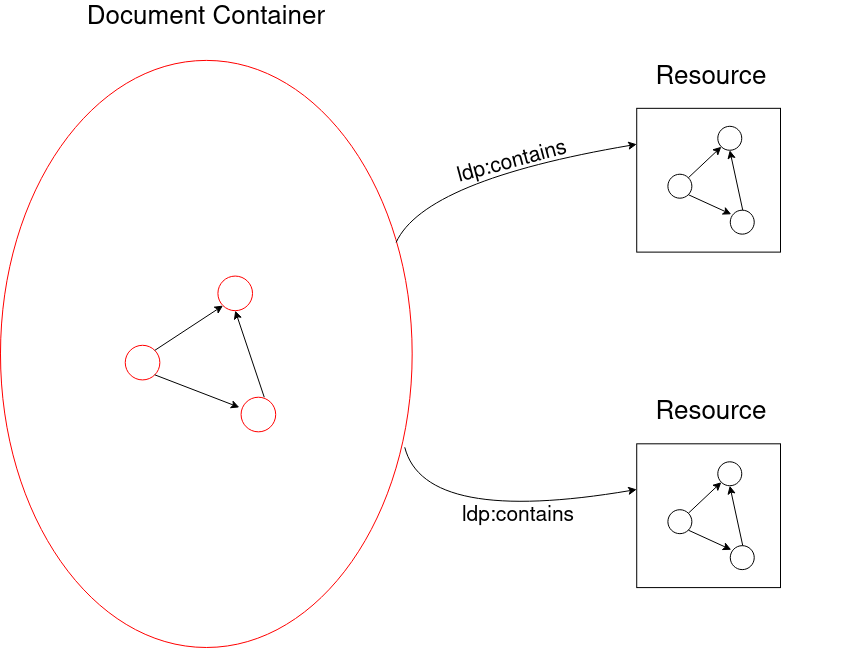
\includegraphics[width=0.60\textwidth]{images/background/ldp-bc.png}}\\
\noindent Direct Containers, or LDP-DCs, are a specialization of a Basic Container. The LDP-DC can make assertions, called membership triples, on resources withing the container. These assertions, which use domain-specific vocabulary, are made as part of the creation process for resources placed in the container. The membership triples do not need to refer to the container resource - these can refer to other resources as well. The figure below illustrates a LDP Basic Container containing movies, and a LDP Direct Container containing documents (images, movies, ..) where the actor is depicted, illustrated through the predicate \texttt{foaf:depicton}. \\
\phantom{kkk|||}{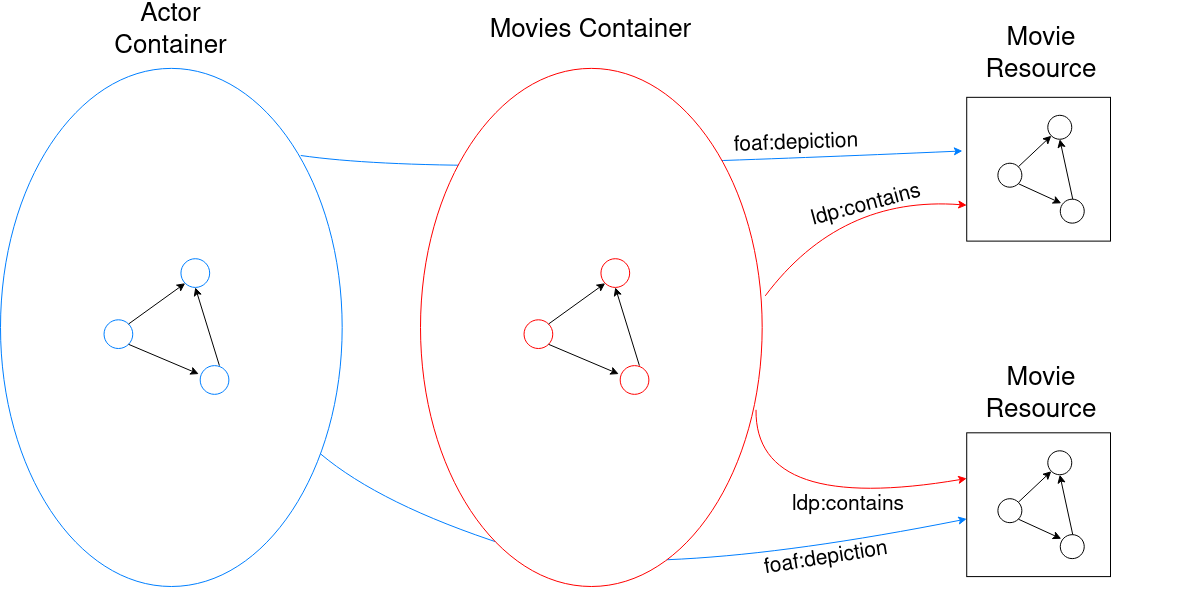
\includegraphics[width=0.9\textwidth]{images/background/ldp-dc.png}}\\

\noindent \textit{Source}: \url{https://www.w3.org/TR/ldp-primer/}
\end{formal}

\newpage

\section{Macaroons}
\label{sec:macaroons}
Macaroons are a type of authorization credential developed for decentralized distributed systems. This section gives some background on why macaroons were developed, followed by the technical details of how they work. As will become clear, macaroons offer many advantages in an inherently decentralized system such as Solid. Macaroons will form an important part of the solutions proposed by this thesis, and thus warrant some extensive background information.

\subsection{Introduction}
\label{sec:macaroons-intro}
Macaroons were developed at Google in \citeyear{macaroons} by \citeauthor{macaroons}. They were created to solve a common authorization problem, for which no sufficient solutions existed yet at the time. In 2014, the Cloud was an emerging technology which began to see widespread adoption. In the Cloud, a microservices architecture is often used, where a piece of software consists of multiple, smaller services. This architecture style has many advantages, such as improved scalability and testability, but it also comes with many challenges regarding authentication and authorization.

In particular, services operated by different owners / stakeholders are often used (for example, using third-party APIs), which necessitates sharing data across multiple trust domains. However, existing solutions are often not sufficient for solving this problem. A very commonly used authentication / authorization mechanism is bearer tokens. Bearer tokens act as a proof that the bearer of the token should have access to a particular resource. However, this implies that anyone able to steal the token can also get access to the resource. Other mechanisms, such as DPoP (see section \ref{sec:dpop}), rely on public-key cryptography, which comes with a high computational cost.

To tackle these challenges, macaroons were introduced. Macaroons are similar to bearer tokens, but with some key differences. Firstly, macaroons introduce a concept called \textit{caveats}. Caveats are requirements which the request to which the macaroon is attached must fulfill in order for the macaroon to be valid. These caveats are embedded in macaroons and cannot be removed thanks to the use of \acrshort{HMAC} signatures. Examples of caveats are:
\begin{enumerate}
    \itemsep0.1em 
    \item \texttt{user = jesse}
    \item \texttt{ip = 193.190.253.145}
    \item \texttt{time < 1649081943}
    \item \texttt{@google.com logged-in as jesse.geens@gmail.com}
\end{enumerate}

As can be seen from the examples, there are two types of caveats. The first type of caveats is called \textit{first-party caveats}. These are caveats that can be checked locally by the server receiving the request. In the example, caveats 1, 2 and 3 are first-party caveats. 
The second type of caveats are \textit{third-party caveats}. These are caveats which must be validated by a third-party server. This is done by returning a so-called \textit{discharge macaroon}. The discharge macaroon is handed out by the third-party server and proves to the first-party server that the embedded caveat is indeed fulfilled. In the example, the fourth caveat is a third-party caveats. These discharge macaroons can in turn also contain additional caveats.

An additional important property of macaroons is called \textit{decentralized delegation}. Often, a service also depends on another service to perform some of its work. Traditionally, service A has a token only valid for service A, and cannot safely transfer its token to another service. Solutions, such as the OAuth On-Behalf-Of flow exist, but these require a lot of communication between the service and the token endpoint. With decentralized delegation, services can give other services also a valid macaroon, with at most the same caveats. A service can also further attenuate the macaroon before handing it off. Finally, macaroons can also be sealed, which makes them unable to be passed along. 

All of this is made possible by the structure of macaroons, which is explained in the next section. Macaroons use \gls{HMAC}, which is computationally very efficient.

\subsection{Construction of macaroons}
Macaroons work in a fashion somewhat similar to blockchains. Macaroons are made up of a chain of messages, the caveats. These messages are used to form a chain of \gls{HMAC} values, of which only the terminal value will be stored in the macaroon. This final value acts as the signature, and can be recalculated by the macaroon-issuing service to verify its authenticity. 

The first message of a macaroon is a (public) \textit{key identifier}. This identifier maps to a secret root key. This root key is used to generate the first signature such that: $$sig_1 = \text{HMAC}(K_r, \text{msg-id})$$
with $K_r$ the secret root key, and $\text{msg-id}$ the first message. The next signature is then calculated as: $$sig_2 = \text{HMAC}(sig_1, C_1)$$
which is then done until all caveats have been incorporated. By keeping the root key secret, the signature of a macaroon cannot be forged. However, the identifier of the root key is needed to ensure that the target service knows which root key to use for signature verification. This mechanism is illustrated in figure \ref{fig:macaroon-hash-chain}.

Since the final signature is visible, macaroons can be further attenuated by the service that makes requests: a new caveat $C_k$ can be added by generating a new signature $sig_{k+1} = \text{HMAC}(sig_k, C_k)$. 

\begin{figure}[H]
     \centering
     \begin{subfigure}[b]{0.45\textwidth}
         \centering
         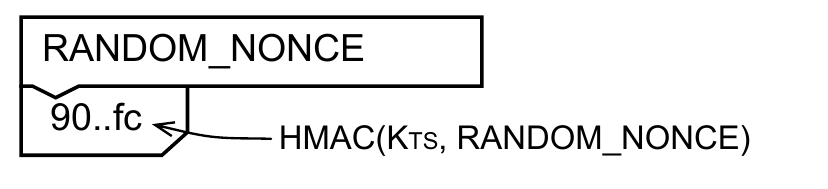
\includegraphics[width=\textwidth]{images/macaroons/basic-macaroon.png}
         \caption{$sig_1$, based on a random nonce (identifier) and the root key}
         \label{fig:macaroon-sig-1}
     \end{subfigure}
     \hfill
     \begin{subfigure}[b]{0.45\textwidth}
         \centering
         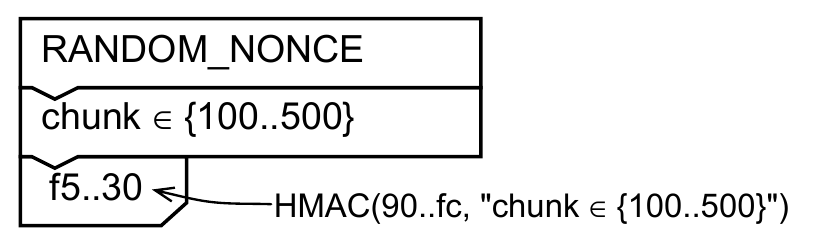
\includegraphics[width=\textwidth]{images/macaroons/macaroon-single-caveat.png}
         \caption{$sig_2$, based on a caveat and $sig_1$}
         \label{fig:macaroon-sig-2}
     \end{subfigure}
        \caption{Illustration of the macaroon signature composition. Source: \citet{macaroons}}
        \label{fig:macaroon-hash-chain}
\end{figure}

\setlength{\abovedisplayskip}{7pt}
\setlength{\belowdisplayskip}{7pt}

Third-party caveats are more difficult to implement. As explained in the previous section, third-party caveats are caveats that must be \textit{discharged} by a third-party server. This is realised using \textit{holder-of-key proofs}. In order to fulfill a third-party caveat, a service must also include a discharge macaroons that acts as a proof that the caveat is fulfilled. As these discharge macaroons are also macaroons, they also have a key identifier. However, in the case of discharge macaroons, this key identifier's purpose is not only to encode which root key was used - it also embeds the predicate that must be verified by the third party.

The way this is realised is by having the first-party server create a new root key for the discharge macaroon. This root key is encrypted with the third-party server's public key. When the requesting application receives the encrypted root key, it can pass it on to the third party server, which generates a new discharge macaroon by decrypting the root key and verifying the embedded requirements. The third-party caveat in the original macaroon contains a key identifier pointing to this root key, as well as the location of the third party server and an encrypted copy of the root key. This copy is encrypted with the current signature of the macaroon, so that it can be decrypted when the macaroon is being validated.
This is illustrated graphically in figure \ref{fig:macaroon-third-party-caveats}.

\begin{figure}[H]
     \centering
     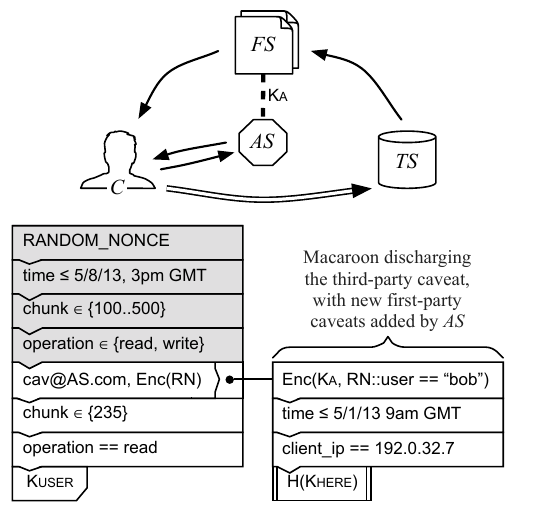
\includegraphics[width=0.75\textwidth]{images/macaroons/third-party-caveat.png}
     \caption{Illustration of third-party caveats and the linked discharge macaroons. The macaroon is issued by TS (grey), extended with additional caveats by FS (white, left), one of which includes a third-party caveat to service AS. K$_A$ is AS's public key. Source: \citet{macaroons}}
     \label{fig:macaroon-third-party-caveats}
\end{figure}

% \subsection{Advantages and limitations}
